\section{Neural Networks}
\label{sec:neural_networks}
Neural Networks are a learning representation which the goal is to approximate some function \( f^* \). Data collected from an environment encodes an underlying function \( \mathrm{\mathbf{y}} = f^*(\mathrm{\mathbf{x}}) \) that maps an input \( \textbf{x} \) to an output \( \mathrm{\mathbf{y}} \), which may be a category from a classifier or a continue value in regression problems. The neural network defines an approximate mapping \( \mathrm{\mathbf{y}} = f(\mathrm{\mathbf{x}};\boldsymbol{\theta}) \), by learning the values of the parameters \(\boldsymbol{\theta}\), which result in the best function approximation. Figure \ref{fig:ann} shows a neural network and an artificial neuron in detail.

\begin{figure}[!htbp]
\centering
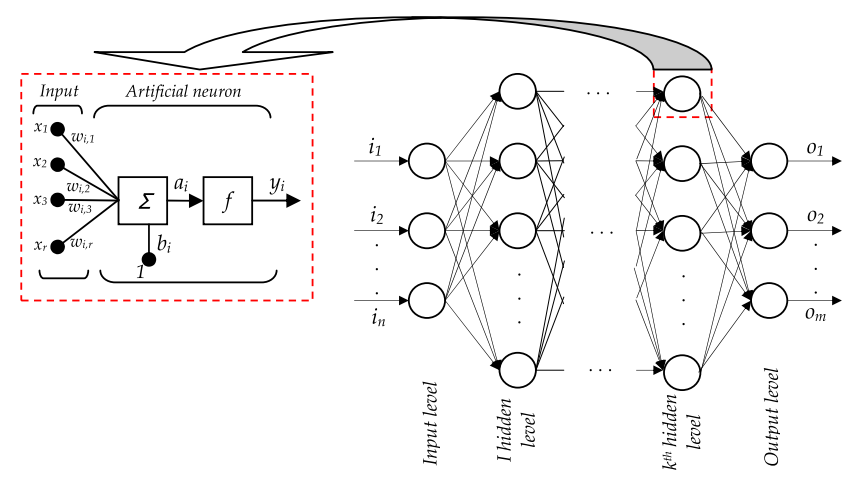
\includegraphics[width=0.8\textwidth]{Cap3/ann}
\caption{An artificial neuron within a feed forward artificial neural network \cite{dejan12}. }
\label{fig:ann}
\end{figure}

These networks are typically represented by composing together many different functions, which are associated with a directed acyclic graph, by describing a computational model. For example, we might have three layers (each of them representing a function \( f^{(1)}, f^{(2)} \), and \(f^{(3)} \)), connecting in a chain and resulting in a final representation \( f(\mathrm{\mathbf{x}}) = f^{(3)}(  f^{(2)} ( f^{(1)}(\mathrm{\mathbf{x}}))) \).

During a neural network training, the objective is to adjust \(f(\mathrm{\mathbf{x}})\) to match \(f^{*}(\mathrm{\mathbf{x}})\), by using the training dataset, which provides noisy examples of \(f^{*}(\mathrm{\mathbf{x}})\) evaluated in different points. The training examples directly specify what the output layer must do at each point \(\mathrm{\mathbf{x}}\), but the learning algorithm must decide how to use all layers to produce this desired output \cite{Goodfellow-et-al-2016}.

\subsection{A Neuron}\label{sec:neuron}

The idea of a neural network starts in the concept of a neuron. Figure \ref{fig:neurondetail} illustrates it in detail.

\begin{figure}[!htbp]
	\centering
	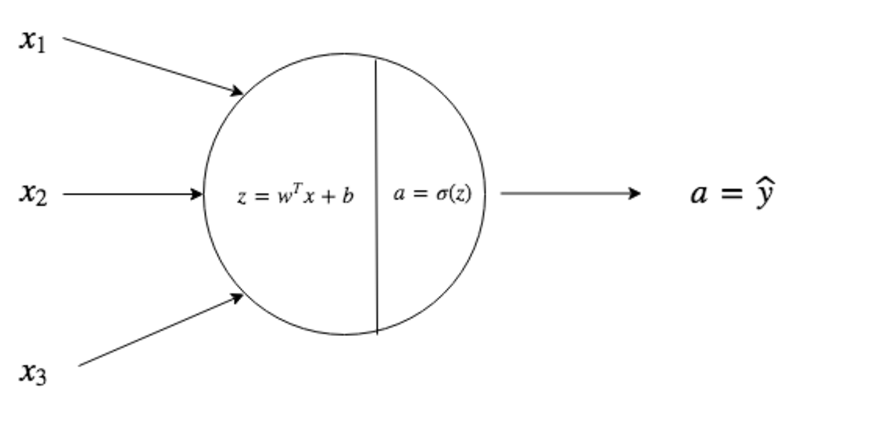
\includegraphics[width=0.8\textwidth]{Cap3/neurondetail.eps}
	\caption{An artificial neuron in detail.}
	\label{fig:neurondetail}
\end{figure}

In a neuron, the first operation is the product between inputs and the respective weights, which represents how much each input signal will influence the computation of that neuron. The core idea of a neural network is calculate the value of those weights in order to generate a better representation of the data generator distribution.

To this linear combination, it's added a bias value, which purpose is to add the capacity of neuron representation by translation, due to the fact this value doesn't rely on the inputs. Figure \ref{fig:bias} shows how weights and bias affect the function representation, described by equation \ref{eq:neuronequation}.


\begin{equation}
z = w^{T}x + b
\label{eq:neuronequation}
\end{equation}



\begin{figure}[!htbp]
	\centering
	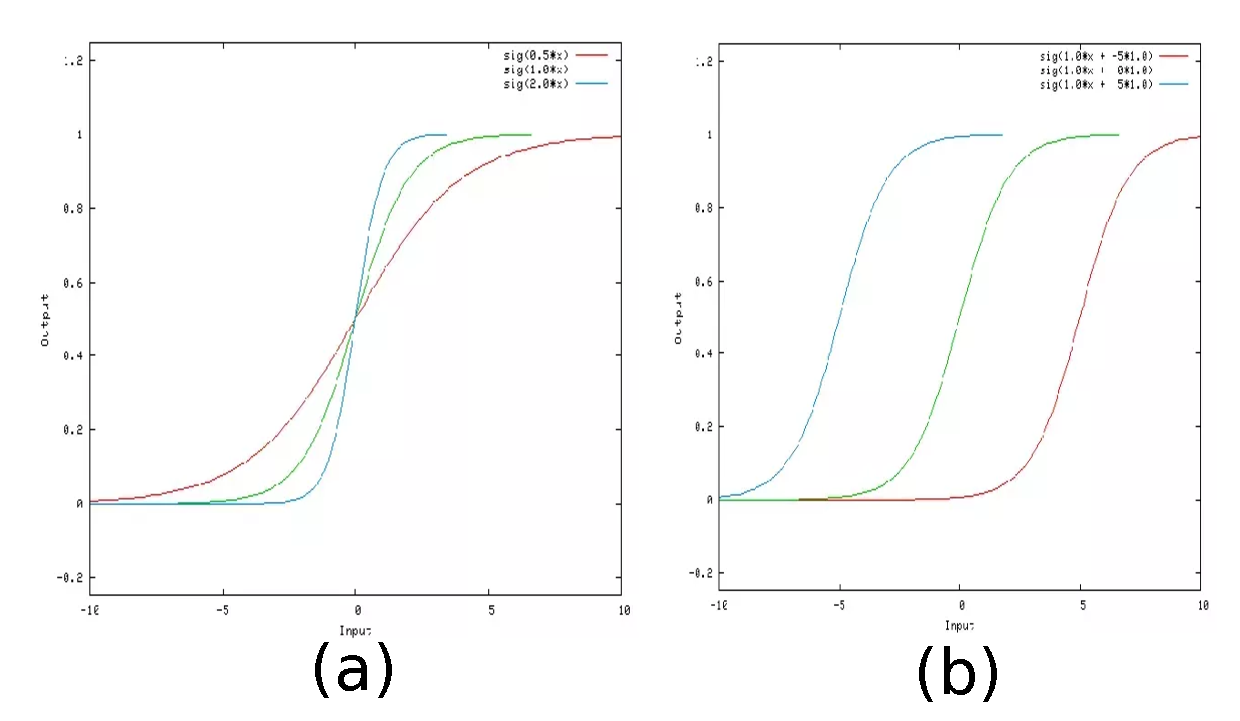
\includegraphics[width=0.9\textwidth]{Cap3/bias.eps}
	\caption{Function representation: in (a), we have a sigmoid function where weights vary. In (b), the same sigmoid but only bias varies.}
	\label{fig:bias}
\end{figure}

The final operation from a neural is the activation function computed using the linear combination as input. In the context of neural networks, this is a non-linear function whose purpose is add the neuron's capacity of representation. Without this idea, the network would be only able to learn linear functions, which will result in poor representation of complex data distributions. Equation \ref{eq:neuronactivation} shows the neuron activation. These functions will be described deeper in section \ref{sec:activationfunction}.

\begin{equation}
a = \sigma({z})
\label{eq:neuronactivation}
\end{equation}


\subsection{Neural Network Representation}

A neural network is a combination of neurons in several layers. It's basically a directed acyclic graph (DAG) where each node performs the operations described in subsection \ref{sec:neuron}. Figure \ref{fig:neuralnetworkrepresentation} shows the representation of a neuron.

\begin{figure}[!htbp]
	\centering
	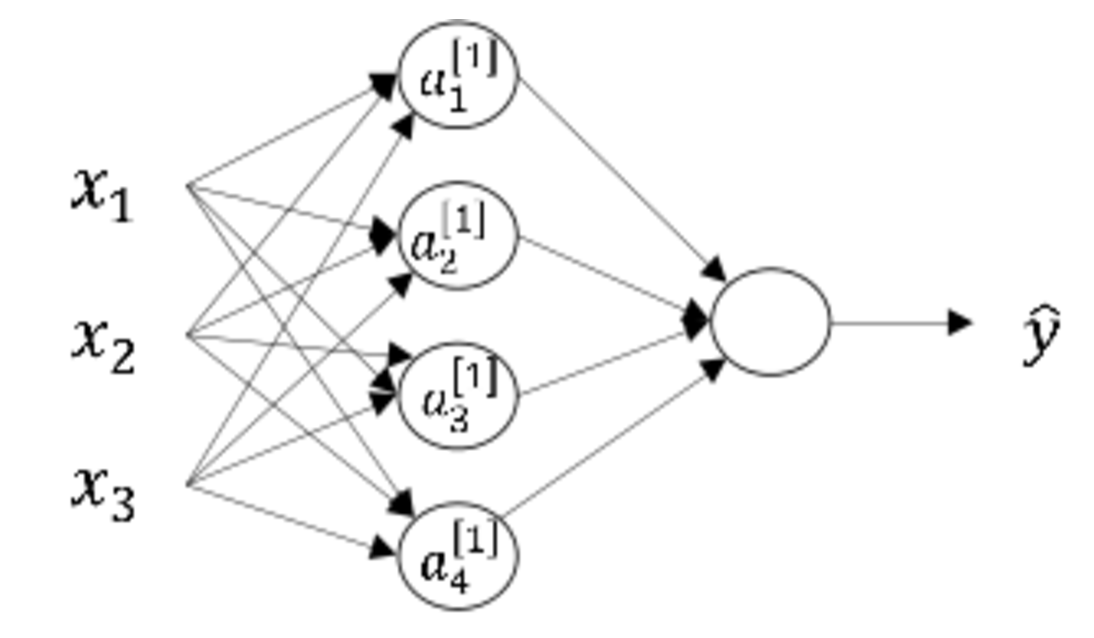
\includegraphics[width=0.7\textwidth]{Cap3/neuralnetworkrepresentation.eps}
	\caption{Neural Network representation.}
	\label{fig:neuralnetworkrepresentation}
\end{figure}

It is worth to mention the math notation used in this work. The neuron $a^{j}_{i}$ represents the $i^{th}$ neuron in the $j^{th}$ layer of network.

The flow of a input tensor in a neural network occurs in the following manner: first, neurons from the same layer performs its calculations. Then, the output of them will serve as input of the next layer. This sequence will keep going until reach the output layer. Equations \ref{eq:nn_begin} to \ref{eq:nn_final} represent the flow from Figure \ref{fig:neuralnetworkrepresentation}.


\begin{align}\label{eq:nn_begin}
z^{[1]} = W^{[1]}x + b^{[1]}\\
a^{[1]} = \sigma(z^{[1]})\\
z^{[2]} = W^{[2]}a^{[1]} + b^{[2]}\\
a^{[2]} = \sigma(z^{[2]})
\label{eq:nn_final}
\end{align}

$W^{i}$ and $b^{i}$ are defined, respectively, as:

\begin{align}
W^{[i]} = \begin{bmatrix}
w^{T[i]}_1 & w^{T[i]}_2 & \dots & w^{T[i]}_n
\end{bmatrix} \\
b^{[i]} = \begin{bmatrix}
b^{[i]}_1 & b^{[i]}_2 & \dots & b^{[i]}_n
\end{bmatrix}
\end{align}

In general, we can represent a layer $i$ recursively as:

\begin{align}
z^{[i]} = W^{[i]}a^{[i-1]} + b^{[i]}\\
a^{[i]} = \sigma(z^{[i]})
\end{align}


The first layer of a neural network is called \textbf{input layer} and represents its inputs. The last layer is the \textbf{output later} and represents its outputs. All layers between those are \textbf{hidden layers}. The greater is the number of layers, the deeper the network is.

\subsection{Vectorization}\label{sec:vectorization}

Vectorization is a technique where a network calculates the output of several examples in a batch at the same time, instead of calculate them sequentially. Basically, we consider as input:

\begin{align}
X = \begin{bmatrix}
x^{T}_1 & x^{T}_2 & \dots & x^{T}_n
\end{bmatrix}
\end{align}

Therefore, the network layers' equations change to:

\begin{align}
Z^{[i]} = W^{[i]}A^{[i-1]} + b^{[i]}\\
A^{[i]} = \sigma(Z^{[i]})
\end{align}

Using vectorized implementations the network can explore better Single Instruction Multiple Data (SIMD) architectures and then speedup learning.

\section{Activation Functions}\label{sec:activationfunction}
As described in subsection \ref{sec:neuron}, an activation function uses the linear combination as input to give a non-linear representation and the improve network learning capacity. Without this, it only is able to represent linear functions.

There are several activation functions. We will describe the most common used in deep learning research.

\subsection{Logistic Sigmoid}

Equation \ref{eq:sigmoid} shows the logistic sigmoid function.

\begin{equation}
\sigma(z) = \frac{1}{1 + e^{-z}}
\label{eq:sigmoid}
\end{equation}

This function is commonly used to produce the parameter of a Bernoulli distribution because its range is (0,1). Furthermore, it saturates when its argument is very positive or very negative, meaning the function becomes very flat and insensitive to small changes in its input \cite{Goodfellow-et-al-2016}. Figure \ref{fig:sigmoid} illustrates the logistic sigmoid function.

\begin{figure}[!htbp]
	\centering
	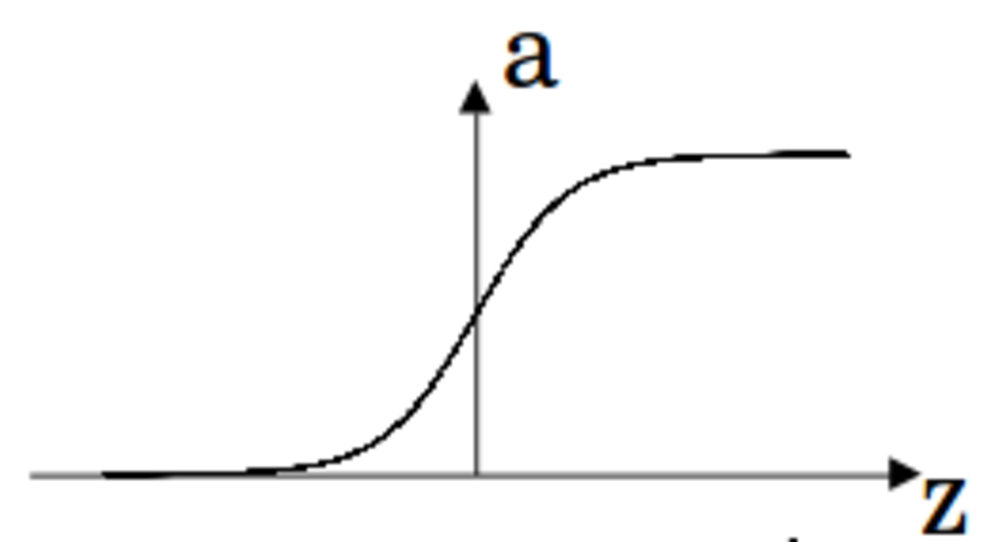
\includegraphics[width=0.7\textwidth]{Cap3/sigmoid.eps}
	\caption{Illustration of Sigmoid function.}
	\label{fig:sigmoid}
\end{figure}

\subsection{Hyperbolic Tangent}

Equation \ref{eq:tanh} shows hyperbolic tangent ($tanh$).


\begin{equation}
tanh(z) = \frac{e^{z} - e^{-z}}{e^{z} + e^{-z}}
\label{eq:tanh}
\end{equation}

It is close related to logistic function, because:

\begin{equation}
tanh(z) = 2\sigma(2z) - 1
\label{eq:tanhsigmoid}
\end{equation}

Hyperbolic tangent is considered a sigmoidal activation function as well, but typically performs better than sigmoid. It resembles the identity function more closely due to its symmetry in $x$ axis. Train a neural network with this activation function resembles a linear model when the input can be kept small, which makes training easier.

Figure \ref{fig:tanh} illustrates hyperbolic tangent.

\begin{figure}[!htbp]
	\centering
	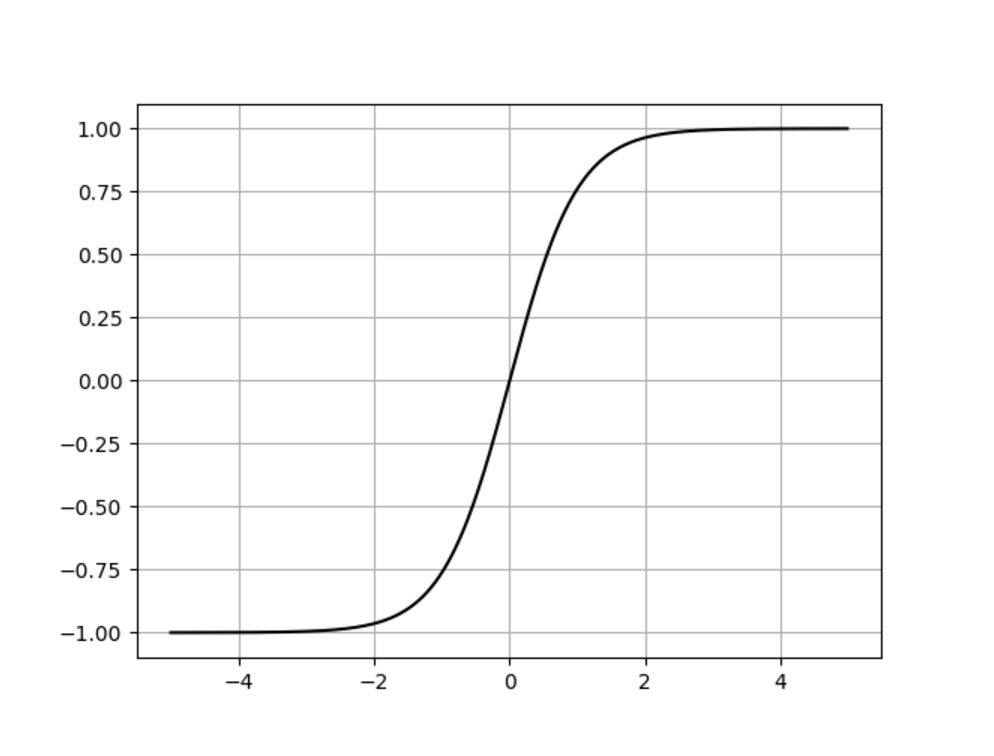
\includegraphics[width=0.7\textwidth]{Cap3/tanh.eps}
	\caption{Illustration of $tanh$ function.}
	\label{fig:tanh}
\end{figure}


\subsection{Rectified Linear Unit - ReLU}

Rectified Linear Unit is a activation function very similar with a linear unit. It is described by equation \ref{eq:relu}:

\begin{equation}
g(z) = max(0,z)
\label{eq:relu}
\end{equation}

The only difference between a linear unit and a rectified linear unit is
that a rectified linear unit outputs zero across half its domain. This makes the
derivatives through a rectified linear unit remain large whenever the unit is active.
The gradients are not only large but also consistent. The second derivative of the
rectifying operation is 0 almost everywhere, and the derivative of the rectifying
operation is 1 everywhere that the unit is active. This means that the gradient
direction is far more useful for learning than it would be with activation functions
that introduce second-order effects \cite{Goodfellow-et-al-2016}. Figure \ref{fig:relu} illustrates this activation function.

\begin{figure}[!htbp]
	\centering
	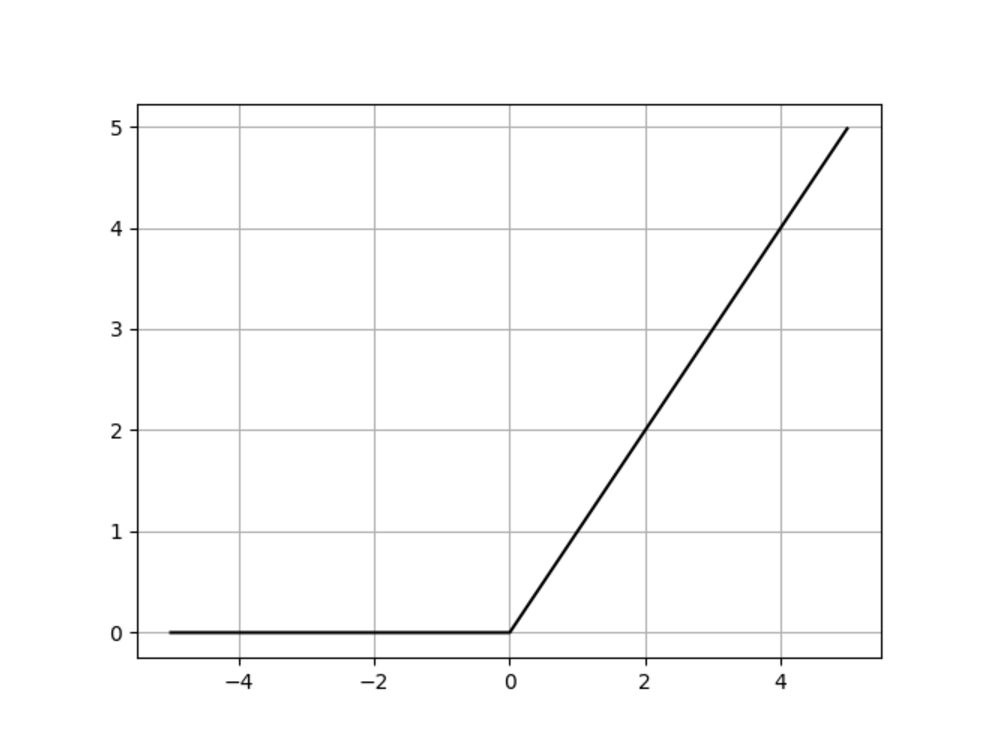
\includegraphics[width=0.7\textwidth]{Cap3/relu.eps}
	\caption{Illustration of ReLU function.}
	\label{fig:relu}
\end{figure}

\cite{glorot2011a} motivate rectified linear units from
biological considerations. The half-rectifying nonlinearity was intended to capture
these properties of biological neurons: 
\begin{itemize}
\item For some inputs, biological neurons are
completely inactive. 
\item For some inputs, a biological neuron’s output is proportional
to its input. 
\item Most of the time, biological neurons operate in the regime where
they are inactive (i.e., they should have sparse activations).
\end{itemize}

\subsection{Leaky ReLU}

One drawback to rectified linear units is that they cannot learn via gradient-based methods on examples for which their activation is zero. Leaky ReLU \cite{leakyrelu} is a
generalization of rectified linear units guarantee that they receive gradient everywhere.

Equation \ref{eq:leakyrelu} represents the Leaky ReLU activation.


\begin{equation}
g(z) = max(\alpha z,z) 
\text{, where } \alpha \in (0,1)
\label{eq:leakyrelu}
\end{equation}

Rectified linear units and all generalizations of them are based on the
principle that models are easier to optimize if their behavior is closer to linear. Figure \ref{fig:leakyrelu} illustrates this activation function.


\begin{figure}[!htbp]
	\centering
	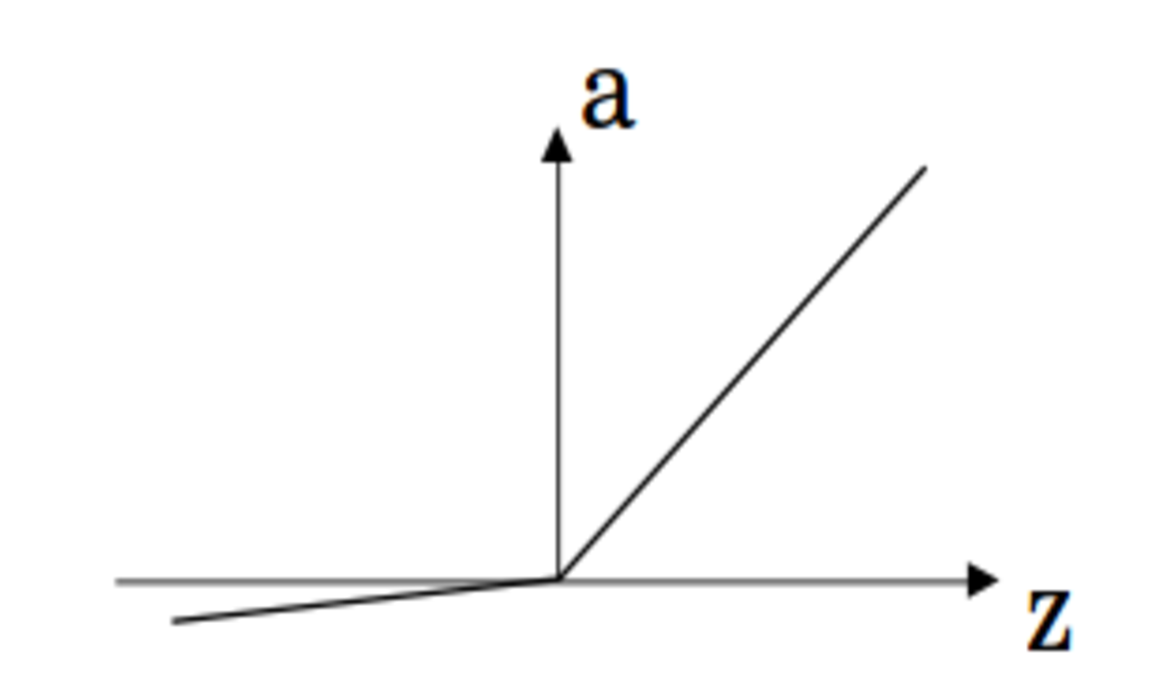
\includegraphics[width=0.7\textwidth]{Cap3/leakyrelu.eps}
	\caption{Illustration of leaky ReLU function.}
	\label{fig:leakyrelu}
\end{figure}


\section{Cost Function}

In the context of neural networks, gradient-based algorithms are broadly used, especially those based on the backpropagation idea \cite{hinton88}. The purpose of these algorithms are to propagate the gradient of a cost function through the whole network, in order to minimize the cost function. Most modern neural networks perform this optimization strategy, by using maximum likelihood, i.e. the cross-entropy between the training data and the model distribution:

\begin{equation}
J(\boldsymbol{\theta}) = -\mathbb{E}_{\mathrm{\mathbf{x}},\mathrm{\mathbf{y}}\sim \hat{p}_{data}}\log{p_{model}(\mathrm{\mathbf{y}} | \mathrm{\mathbf{x}})}
\label{eq:cost_function_ml}
\end{equation}

In this work, we used the mean squared error loss function, in order to fit data distributions. Indeed, we may show that both cost functions are closely related. Let us consider normally distributed errors:

\begin{equation}
{p_{model}(\bvec{y} | \bvec{x})} = \mathcal{N}( \bvec{y}; f (\bvec{x}; \boldsymbol{\theta}), \sigma^{2}\bvec{I})
\label{eq:errors}
\end{equation}
where \(f (\bvec{x}; \boldsymbol{\theta})\) and \(\sigma^{2}\bvec{I}\)  are the mean and covariance of this distribution. By substituting Eq. \eqref{eq:errors} in Eq. \eqref{eq:cost_function_ml}:

\begin{equation}
J(\boldsymbol{\theta}) = \frac{1}{2}\mathbb{E}_{\bvec{x},\bvec{y}\sim \hat{p}_{data}} \lVert \bvec{y} - f (\bvec{x}; \boldsymbol{\theta}) \rVert ^{2} + const
\label{eq:cost_function_expectation}
\end{equation} 

The constant term does not depend on \( \boldsymbol{\theta} \) and may be dropped. By explicitly evaluating the expectation in Eq. \eqref{eq:cost_function_expectation}, we arrive at the mean squared error cost function:

\begin{equation}
J(\boldsymbol{\theta}) = \frac{1}{2m} \sum^{m}_{i} \lVert y_{i} - f (\bvec{x}; \boldsymbol{\theta}) \rVert ^{2}
\end{equation}

It can be shown that maximum likelihood estimator is the best estimator asymptotically, when the number of samples $m$ tends to infinity, in terms of its rates of convergence as $m$ increases. Furthermore, this estimator has the property of consistency, under certain conditions that must be satisfied by the data distribution, and efficiency, in terms of achieve lower generalization errors.	

\section{Gradient Descent}\label{gradientdescent}

The objective of a neural network training is find the parameters $W$ and $b$ that approximates the function represented by itself and the data generator distribution, by minimizing the cost function established. In math terms, it means:

\begin{equation}
(W^{*},b^{*}) = \argmin_{W,b}J(W, b, x)
\end{equation}


The Gradient Descent technique is a iterative method that calculates the derivative of the loss function and applies them as learning updates according to a learning rate factor, $\alpha$, previously set. Figure \ref{fig:gradientdescent} illustrates the application of this technique in the context of two variables.

\begin{figure}[!htbp]
	\centering
	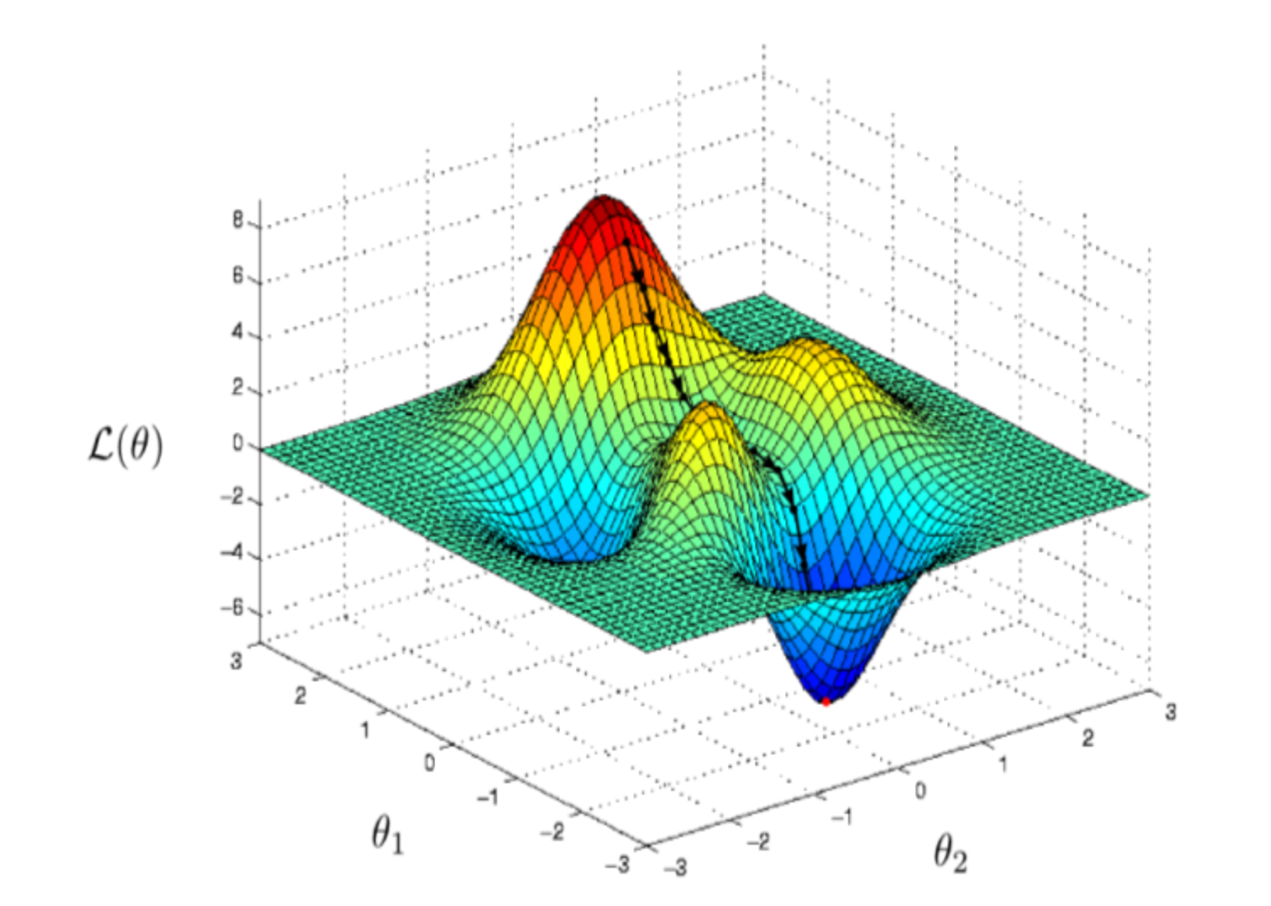
\includegraphics[width=0.7\textwidth]{Cap3/gradientdescent.eps}
	\caption{Illustration of gradient descent in a two variables optimization
	\cite{tgilharco}.
	}
	\label{fig:gradientdescent}
\end{figure}


As an example, given the following cost function (where $m$ is the number of samples, $\hat{y}$ is the prediction of the network and $y$ is the ground-truth):

\begin{equation}
J(W,b) = \frac{1}{m}\sum^{n}_{i = 1}\mathcal{L}(\hat{y}, y)
\end{equation}


The gradient with respect of the parameters $W$ and $b$ can be given by:

\begin{align}
\frac{\partial{J(W,b)}}{\partial{W}} = \frac{1}{m}\sum^{n}_{i = 1}\frac{\partial{\mathcal{L}(\hat{y}, y)}}{\partial{W}}\\
\frac{\partial{J(W,b)}}{\partial{b}} = \frac{1}{m}\sum^{n}_{i = 1}\frac{\partial{\mathcal{L}(\hat{y}, y)}}{\partial{b}}
\end{align}

After these calculations, we are able to apply these gradients using the learning update rule:


\begin{align}
W = W - \alpha\frac{\partial{J(W,b)}}{\partial{W}}\\
b = b - \alpha\frac{\partial{J(W,b)}}{\partial{b}}
\end{align}

These steps are applied iteratively until the function converges to a optimal value. It's important to mention that there are no guarantees the optimization will converge to a global optima, i.e, it is possible to get stuck in local optima. However, in practical applications, this is not a huge problem.

\section{Backpropagation}
In the case described in section \ref{gradientdescent} we computed the gradient directly with respect to parameters $W$ and $b$. However, in neural networks, we have to compute the gradients that correspond to all and layers and not just to the output layer. For this, we need to use the chain rule of calculus.

Let $x$ be a real number, and let $f$ and $g$ both be functions mapping from a real
number to a real number. Suppose that $y = g(x)$ and $z = f (g(x)) = f (y)$. Then
the chain rule states that


\begin{equation}
\frac{dz}{dx} = \frac{dz}{dy}\frac{dy}{dx}
\end{equation}

We can generalizes to vectorial case. Suppose that $\boldsymbol{x} \in \mathbb{R}^{m} , \boldsymbol{y} \in \mathbb{R}^{n}$, $g$ maps from $\mathbb{R}^{m}$ to $\mathbb{R}^{n}$ , and $f$ maps from $\mathbb{R}^{m}$ to $\mathbb{R}^{n}$. If $\boldsymbol{y} = g(\boldsymbol{x})$ and $\boldsymbol{z} = f( \boldsymbol{y})$, then

\begin{equation}
\frac{\partial{z}}{\partial{x_i}} = \sum_{j} \frac{\partial{z}}{\partial{y_{j}}}\frac{\partial{y_{j}}}{\partial{x_{i}}}
\end{equation}
 
It can be generalized more generic in a way that can be applied to tensors:

\begin{equation}
\nabla_{\textbf{X}}z = \sum_{j}(\nabla_\textbf{X}Y_{j})  \frac{\partial{z}}{\partial{Y_{j}}}
\label{eq:backprop}
\end{equation}

The backpropagation takes equation \ref{eq:backprop} recursively, until the gradient is propagated to all layers of the neural network. Algorithm \ref{alg:backprop} \cite{Goodfellow-et-al-2016} shows in a simple way how to apply backpropagation to a deep neural network.

\begin{algorithm}[!htbp]
	\caption{Backward computation for a deep neural network}
	\begin{algorithmic} 
		\STATE After the forward computation, compute the gradient on the output layer:
		\STATE $\boldsymbol{g} \leftarrow \nabla_{\boldsymbol{\hat{y}}}J = \nabla_{\boldsymbol{\hat{y}}}\mathcal{L}(\boldsymbol{\hat{y}},y)$
		\STATE \textbf{for} $k = l, l - 1,
		 \dots, 1$ \textbf{do}
		
		\STATE \hspace{5mm} Convert the gradient on the layer’s output into a gradient into the pre-nonlinearity activation (element-wise multiplication if f is element-wise):
		\STATE \hspace{5mm} $\boldsymbol{g} \leftarrow \nabla_{\boldsymbol{a^{(k)}}}J = \boldsymbol{g} \odot f'(\boldsymbol{a}^{(k)})$
		\STATE \hspace{5mm} Compute gradients on weights and biases:
		\STATE \hspace{5mm} $\nabla_{\boldsymbol{b}^{(k)}}J = \boldsymbol{g}$
		\STATE \hspace{5mm} $\nabla_{\boldsymbol{W}^{(k)}}J = \boldsymbol{g} \boldsymbol{h}^{(k-1)T}$
		\STATE \hspace{5mm} Propagate the gradients w.r.t. the next lower-level hidden layer’s activations:		
		\STATE \hspace{5mm} $\boldsymbol{g} \leftarrow \nabla_{\boldsymbol{h}^{(k - 1)}}J = \boldsymbol{W}^{(k)T}\boldsymbol{g}$
		\STATE \textbf{end for}
	\end{algorithmic}
	\label{alg:backprop}
\end{algorithm}

\section{Optimization Algorithms}
In Deep Learning community, gradient-based optimization is well established. However, in state-of-art research the backpropagation idea had several improvements to make learning better. In this section, we will explore some of these improvements and present the optimizer used in experimentation.

\subsection{Batch, Mini-batch and Stochastic Gradient Descent}
There are ways to use the data in order to apply learning updates. Accordingly to section \ref{sec:vectorization}, using vectorization makes possible to calculate several losses at the same time. However, sometimes the dataset is very large in a way it is costly to apply a single batch several times. On the other side, apply updates using one sample at a time can result in a biased gradient and also can be costly due to the fact we need to apply an update for each sample. Therefore, the batch size can change a lot the learning process.

The Batch Gradient Descent calculates the cost function for each sample in the dataset and only updates the model after all samples have been evaluated. In this way, there are fewer updates and the gradient is more precise, due to the fact we consider several samples to regularize it. So, the training and convergence are more stable. However, this variation of gradient descent can result in local optima convergence and turns to be very slow with large datasets.

The Stochastic Gradient Descent calculates the cost function and updates the model for each samples in dataset. Using this variation, there are more frequent updates which can give feedback about the model fast and result in faster learning to some problems. Furthermore, the noisy update allows exploration in function optimization, avoiding local optima (Figure \ref{fig:batchvsstochastic}). However, there is a high computational cost of applying updates so frequently and the same noise can make hard for the last optimization steps. Equation \ref{eq:sgd} shows the learning update rule for Stochastic Gradient Descent:

\begin{equation}
W = W - \alpha\frac{\partial{J(W,b, x^{(i)})}}{\partial{W}}
\label{eq:sgd}
\end{equation}

\begin{figure}[!htbp]
	\centering
	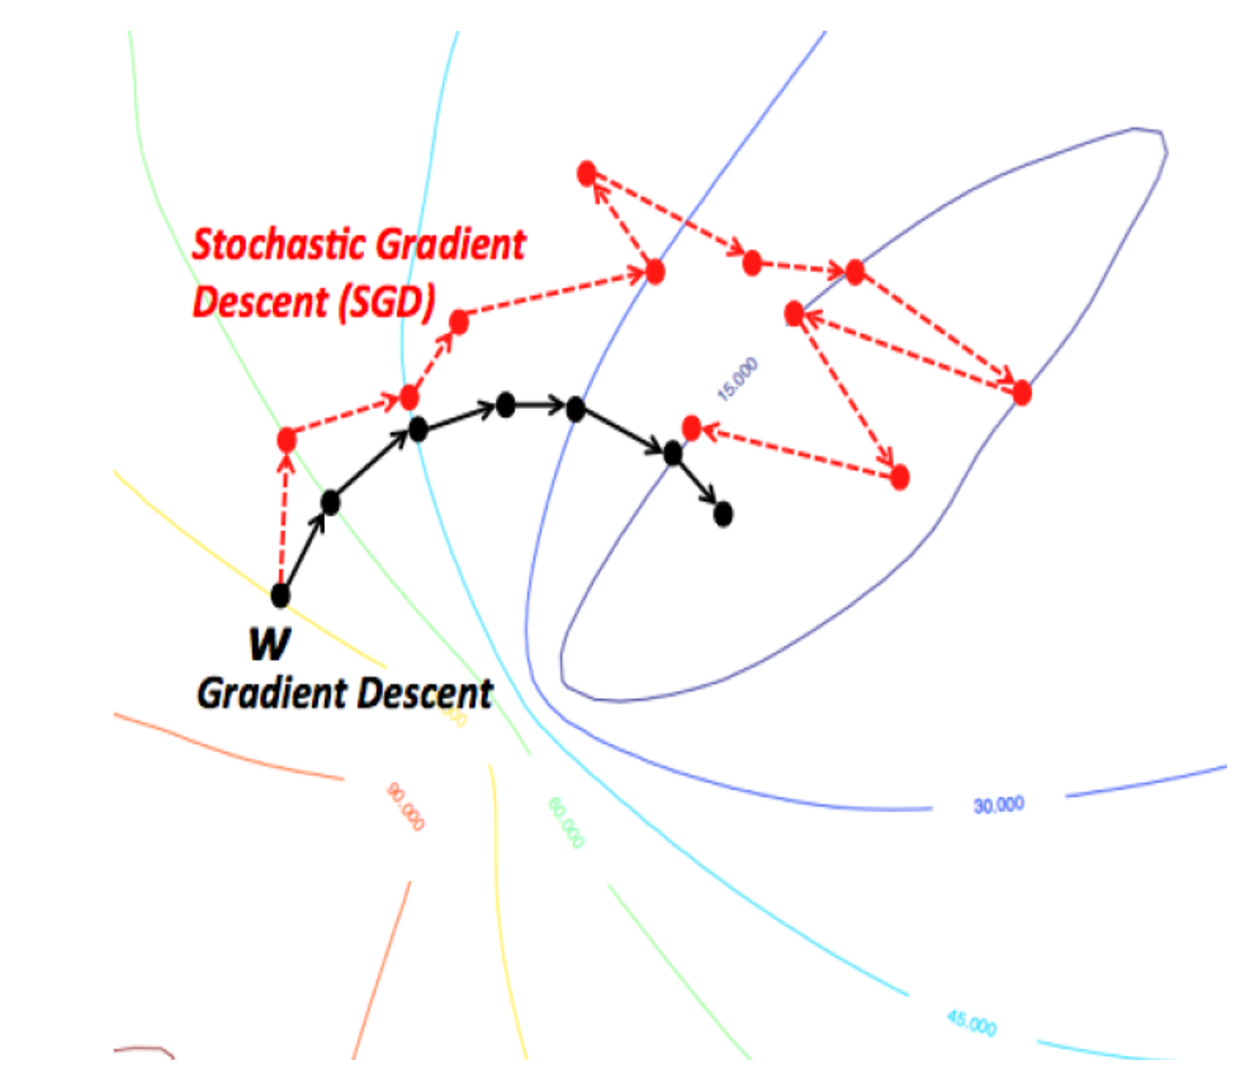
\includegraphics[width=0.8\textwidth]{Cap3/batchvsstochastic.eps}
	\caption{Illustration of 	Stochastic Gradient Descent optimization.
	}
	\label{fig:batchvsstochastic}
\end{figure}


Figure \ref{fig:lossfunctiongdvariants} shows how cost function commonly behaves in each variation of Gradient Descent described.

\begin{figure}[!htbp]
	\centering
	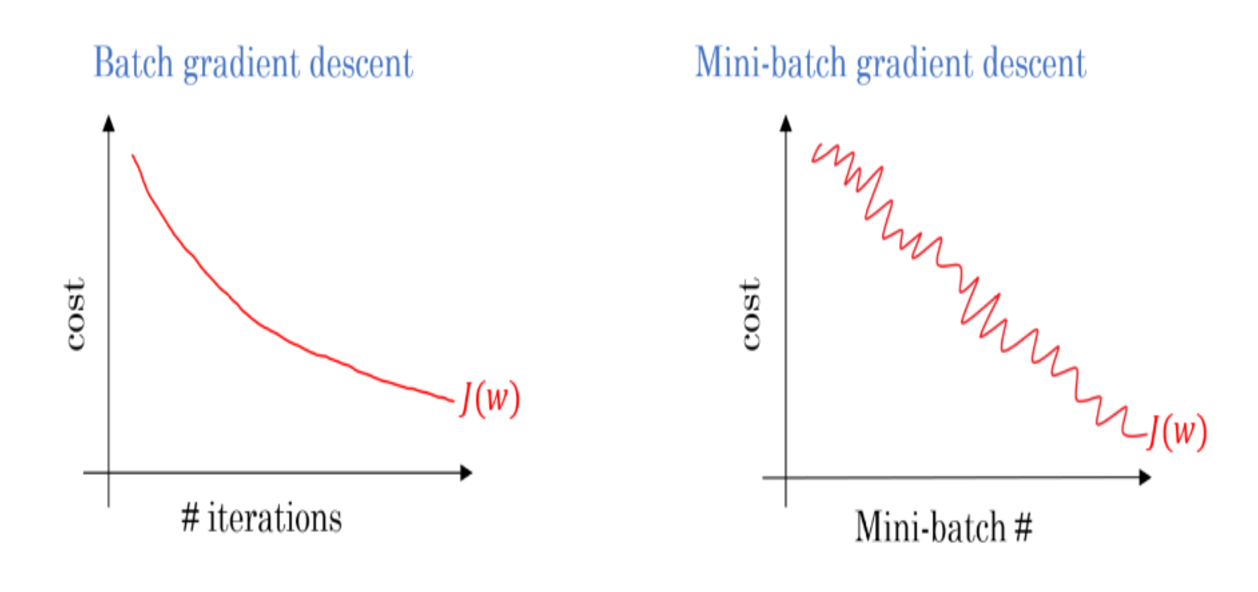
\includegraphics[width=0.8\textwidth]{Cap3/lossfunctiongdvariants.eps}
	\caption{Illustration of how each variation of Gradient Descent commonly behaves.
	\cite{dabbura2017}.
	}
	\label{fig:lossfunctiongdvariants}
\end{figure}



There is a third variant. The Mini-batch Gradient Descent is something in between batch and stochastic variants, where the algorithm splits dataset into small batches and each of them will apply learning updates. This version seeks to find a balance between the robustness of SGD and the efficiency of BGD. It is the most common implementation used in Deep Learning \cite{brownlee2017}. However, the downside of this variation is the fact we need to set a new hyperparameter and tune it manually.



\subsection{Momentum}

Momentum is a technique for accelerating gradient descent that accumulates a velocity vector in directions of persistent reduction in the objective across iterations \cite{Sutskever:2013:IIM:3042817.3043064}. It uses the idea of exponentially weighted moving averages, accumulating gradients for each mini-batch accordingly to a hyperparameter $\beta$. This term will manage how much the last gradient will affect in the final velocity, following Equations \ref{eq:momentum} and \ref{eq:momentum_b}. Momentum aims primarily to solve two problems: poor conditioning of the
Hessian matrix and variance in the stochastic gradient \cite{Goodfellow-et-al-2016}.


\begin{align}\label{eq:momentum}
v_{dW} = \beta v_{dW} + (1 - \beta)dW\\
v_{db} = \beta v_{db} + (1 - \beta)db
\label{eq:momentum_b}
\end{align}

Where $dW$ and $db$ are, respectively:

\begin{align}
dW = \frac{\partial{J(W,b)}}{\partial{W}}\\
db = \frac{\partial{J(W,b)}}{\partial{b}}
\end{align}

Therefore, using Momentum, the learning update is:

\begin{align}\label{eq:momentumupdate}
W = W - \alpha v_{dW}\\
b = b - \alpha v_{db}
\end{align}

The intuition behind Momentum is to filter the gradient, "reinforcing" it in the effective directions and removing the noisy ones. Then, it makes harder to apply learning updates in the wrong direction caused by noise samples. Figure \ref{fig:momentum} shows how Momentum changes Gradient Descent updates.


\begin{figure}[!htbp]
	\centering
	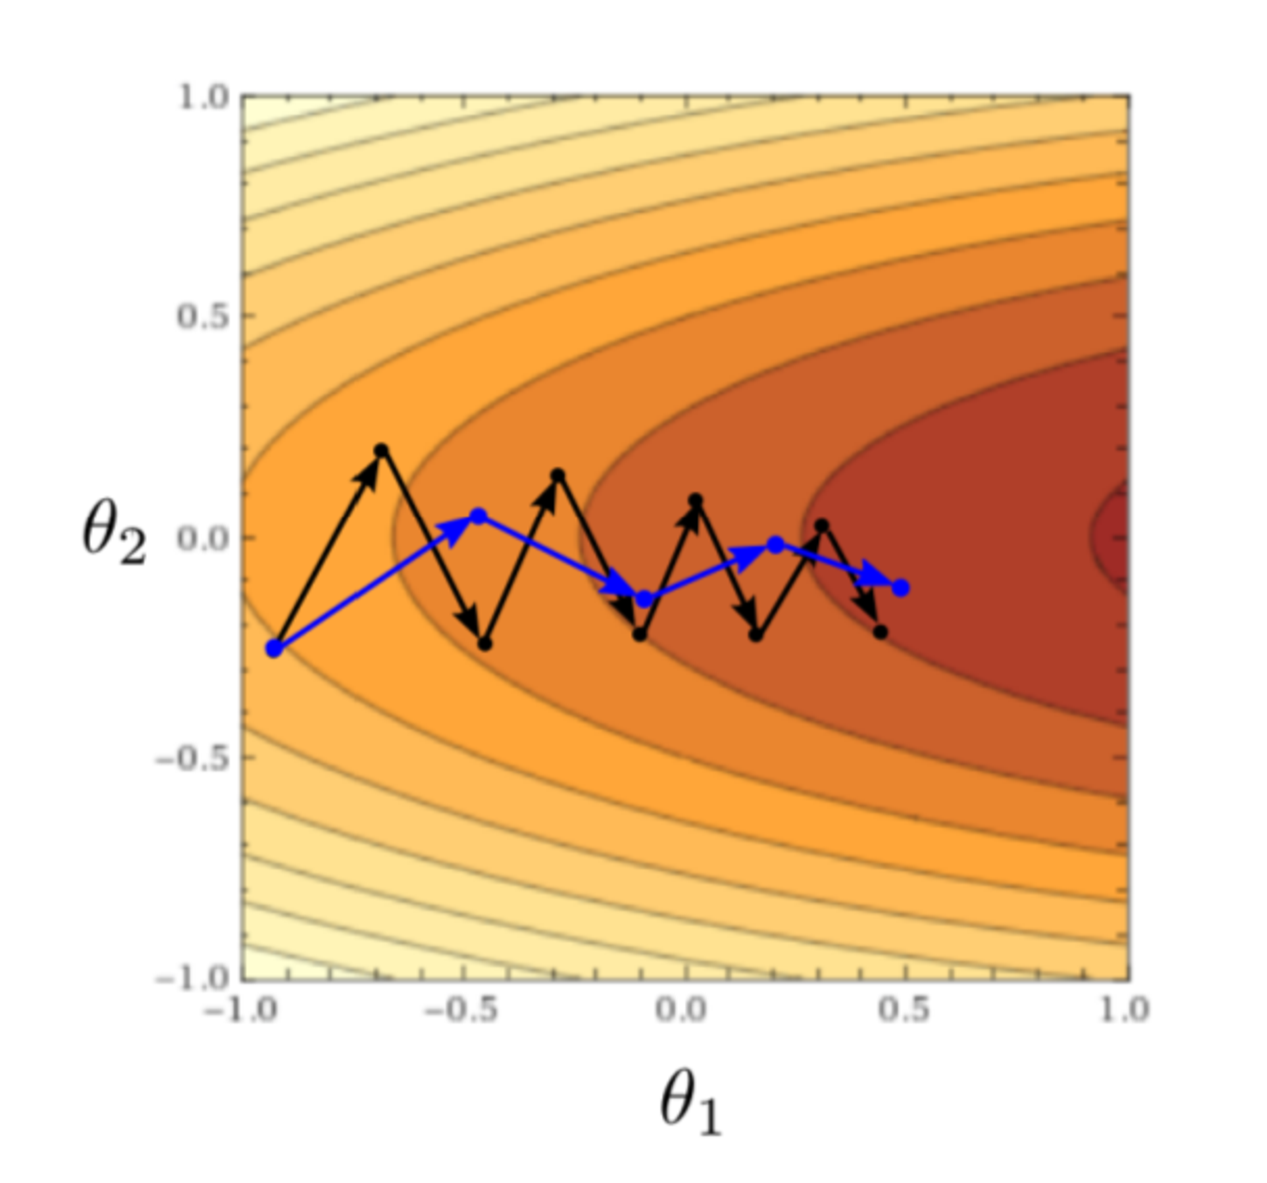
\includegraphics[width=0.8\textwidth]{Cap3/momentum.eps}
	\caption{ Illustration of how Gradient Descent with Momentum (blue arrows) and without it (black arrows)
		\cite{tgilharco}.
	}
	\label{fig:momentum}
\end{figure}

\subsection{RMSProp}

RMSProp \cite{hinton2012} uses the idea of exponentially weighted moving average for gradient accumulation in a non-convex optimization scenario. Instead of using the gradient to update velocity as Momentum does, RMSProp uses the square of this gradient, as shown in Equations \ref{eq:rmsprop} and \ref{eq:rmsprop_b}.


\begin{align}\label{eq:rmsprop}
v_{dW} = \beta v_{dW} + (1 - \beta)dW^2\\
v_{db} = \beta v_{db} + (1 - \beta)db^2
\label{eq:rmsprop_b}
\end{align}

And the learning update changes to normalize the gradient:

\begin{align}\label{eq:rmspropupdate}
W = W - \alpha \frac{dW}{\sqrt{v_{dW}}}\\
b = b - \alpha \frac{db}{\sqrt{v_{db}}}\\
\label{eq:rmspropupdate_b}
\end{align}

This normalization improves the learning stability -- all gradient terms will affect with the same scale. Empirically, RMSProp has been shown to be an effective and practical optimization algorithm for deep neural networks. Algorithm \ref{alg:rmsprop} shows RMSProp idea \cite{Goodfellow-et-al-2016}.


\begin{algorithm}[!htbp]
	\caption{RMSProp Algorithm}
	\begin{algorithmic}
		\REQUIRE Learning rate $\alpha$, decay rate $\beta$
		\REQUIRE Parameters $W$, $b$
		\REQUIRE $\epsilon$ correction for numeric stability 
		\STATE Initialize $v_{dW}$ = $v_{db}$ = 0
		\STATE \textbf{while} stopping criteria not met \textbf{do}
		\STATE \hspace{5mm} Sample a mini-batch of $m$ examples from training set \{$\boldsymbol{x}^{(1)}, \dots, \boldsymbol{x}^{(m)} \}$ with corresponding targets $\boldsymbol{y}^{(i)}$
		\STATE \hspace{5mm} Compute gradient: 
		 $\boldsymbol{g} \leftarrow \nabla_{\boldsymbol{\hat{y}}}J = \frac{1}{m} \nabla_{\boldsymbol{\hat{y}}}\sum_{i = 1}^{m}\mathcal{L}(\boldsymbol{\hat{y}^{(i)}},y^{(i)})$
		 \STATE \hspace{5mm} Accumulate squared gradient: \STATE \hspace{10mm} $v_{dW} = \beta v_{dW} + (1-\beta) g \odot g$ 
		 \STATE \hspace{10mm} $v_{db} = \beta v_{db} + (1-\beta) g \odot g$
		 \STATE \hspace{5mm} Apply updates:
		 \STATE \hspace{10mm} $W = W - \alpha \odot \frac{g}{\sqrt{v_{dW} + \epsilon}}$ 
		 \STATE \hspace{10mm} $b = b - \alpha \odot \frac{g}{\sqrt{v_{db} + \epsilon}}$ 
		\STATE \textbf{end while}
	\end{algorithmic}
	\label{alg:rmsprop}
\end{algorithm}

\subsection{Adam}

The last optimization algorithm idea explored here - and used in experimentations - is Adam \cite{adam2014}. It means ``Adaptive Moments" and combines the idea from Momentum and RMSProp in the following way: it computes the first order momentum of the gradient and rescale with the second order momentum, as shown in Equations \ref{eq:adam_1} and \ref{eq:adam_2}. The use of momentum in combination with rescaling does not have a clear theoretical motivation. 

\begin{align}\label{eq:adam_1}
v_{dW} = \beta_{1} v_{dW} + (1 - \beta_{1})dW\\
u_{dW} = \beta_{2} u_{dW} + (1 - \beta_{2})dW^2
\label{eq:adam_2}
\end{align}

Adam also incorporates a bias correction for both momentum estimates, resulting in lower bias early in training when compared to RMSProp:

\begin{align}
v_{dW} = \frac{v_{dW}}{(1 - \beta_{1}^{t})}\\
u_{dW} = \frac{u_{dW}}{(1 - \beta_{2}^{t})}
\end{align}

Finally, the learning update changes as well:

\begin{align}
W = W - \alpha  \frac{v_{dW}}{\sqrt{u_{dW} + \epsilon}} \\
b = b - \alpha \frac{v_{db}}{\sqrt{u_{db} + \epsilon}}
\end{align}

Therefore, Adam is generally regarded as being fairly robust to the choice of hyperparameters, though sometimes learning rate needs to be changed from the suggested default.  Algorithm \ref{alg:adam} shows Adam idea \cite{Goodfellow-et-al-2016}.


\begin{algorithm}[!htbp]
	\caption{Adam Algorithm}
	\begin{algorithmic}
		\REQUIRE Learning rate $\alpha$ (Suggested default: 0.001)
		\REQUIRE Exponential decay rates for moment estimates, $\beta_{1}$ and $\beta_{2}$
		\REQUIRE Parameters $W$, $b$
		\REQUIRE $\epsilon$ correction for numeric stabilization 
		\STATE Initialize $v_{dW}$ = $v_{db}$ = $u_{dW}$ = $u_{db}$
		\STATE Initialize time step $t$ = 0
		\STATE \textbf{while} stopping criteria not met \textbf{do}
		\STATE \hspace{5mm} Sample a mini-batch of $m$ examples from training set \{$\boldsymbol{x}^{(1)}, \dots, \boldsymbol{x}^{(m)} \}$ with corresponding targets $\boldsymbol{y}^{(i)}$
		\STATE \hspace{5mm} Compute gradient: 
		$\boldsymbol{g} \leftarrow \nabla_{\boldsymbol{\hat{y}}}J = \frac{1}{m} \nabla_{\boldsymbol{\hat{y}}}\sum_{i = 1}^{m}\mathcal{L}(\boldsymbol{\hat{y}^{(i)}},y^{(i)})$
		\STATE \hspace{5mm} $t = t + 1$
		\STATE \hspace{5mm} Update biased first momentum estimate: 
		\STATE \hspace{10mm} $v_{dW} = \beta_{1} v_{dW} + (1-\beta_{1}) g$ 
		\STATE \hspace{10mm} $v_{db} = \beta_{1} v_{db} + (1-\beta_{1}) g$
		\STATE \hspace{5mm} Update biased second momentum estimate:
		\STATE \hspace{10mm} $v_{dW} = \beta_{2} v_{dW} + (1-\beta_{2}) g \odot g$
		\STATE \hspace{10mm} $v_{db} = \beta_{2} v_{db} + (1-\beta_{2}) g \odot g$
		\STATE \hspace{5mm} Correct bias in first moment:
		\STATE \hspace{10mm} $v_{dW} = \frac{v_{dW}}{1-\beta_{1}^{t}} $
		\STATE \hspace{10mm} $v_{db} = \frac{v_{db}}{1-\beta_{1}^{t}} $
		\STATE \hspace{5mm} Correct bias in second moment:
		\STATE \hspace{10mm} $u_{dW} = \frac{u_{dW}}{1-\beta_{2}^{t}} $
		\STATE \hspace{10mm} $u_{db} = \frac{u_{db}}{1-\beta_{2}^{t}} $
		\STATE \hspace{5mm} Apply updates:
		\STATE \hspace{10mm} $W = W - \alpha \odot \frac{v_{dW}}{\sqrt{u_{dW} + \epsilon}}$ 
		\STATE \hspace{10mm} $b = b - \alpha \odot \frac{v_{db}}{\sqrt{u_{db} + \epsilon}}$ 
		\STATE \textbf{end while}
	\end{algorithmic}
	\label{alg:adam}
\end{algorithm}

\section{Weights Random Initialization}
In order to start the learning, it is needed a way to initialize weight parameters. The way these are initialized can affect the convergence and even make it inviable.
Suppose weights are all initialized by zero. No matter what was the input, if all weights are the same, all units in the same hidden layer will receive the same signal, either from the input in forward propagation or from the gradient in backpropagation. 

Therefore, it needs a way for breaking the symmetry. For that, the rule is initialize all weights randomly. It will also break symmetry and increase the entropy in system in way it can gather more information to find local or global minimums.

There are several ways to initialize weights randomly. In this work, we will explore and use Xavier Initialization.


\subsection{Xavier Initialization}

Xavier Initialization \cite{Glorot10} is a method for initialize weights accordingly to the network architecture. 

There are two main problems that arises from bad weight initialization. First, if weights are too small, the signal shrinks as it passes through layers. Second, if they are too large, the signal grows as it passes through layers. Specifically during learning, it will result in vanishing and exploding gradients, respectively.

Xavier Initialization makes sure weights are started in a reasonable range by using a Gaussian distribution with variance given by Equation \ref{eq:xavierinitialization}.

\begin{equation}\label{eq:xavierinitialization}
	\sigma^{2}(W) = \frac{2}{n_{in} + n_{out}}
\end{equation}

Where $n_{in}$ and $n_{out}$ are the number of neurons feeding into it and the result is fed to, respectively. \cite{Glorot10} shows the mathematical development for this equation.

\section{Gradient Descent convergence and learning rate decay}


It is possible to prove the convergence of gradient descent for a specific set of functions.

\newtheorem{gdconv}{Theorem}\label{proof:gdconv}
\begin{gdconv}
	Suppose the function $f : \mathbb{R}^{n} \rightarrow \mathbb{R}$ is convex and differentiable, and that its gradient is Lipschitz continuous with constant $L > 0$, i.e, we have that $\lVert \nabla f(x) - \nabla f(y) \rVert_{2} \leq L\lVert x - y \rVert_{2}$, for any x, y. Then if we run gradient descent for k iterations with a fixed step $t \leq \frac{1}{L}$, it will yield a solution $f^{(k)}$ which satisfies
	
	\begin{equation}
		f(x^{(k)}) - f(x^{(*)}) \leq \frac{\lVert x^{(0)} - x^{*} \rVert^{2}_{2}}{2tk} 
	\end{equation}
	
	where $f(x^{(*)})$ is the optimal value.
\end{gdconv}

The proof of this theorem can be found in \cite{tibshirani2013}. Therefore, using a fixed value for the learning rate, it converges with the rate $O(1/k)$. However, if a large learning rate is chosen, there are no guarantees of convergence. Figure \ref{fig:gddivergence} shows a case of divergence in a one variable optimization.


\begin{figure}[!htbp]
	\centering
	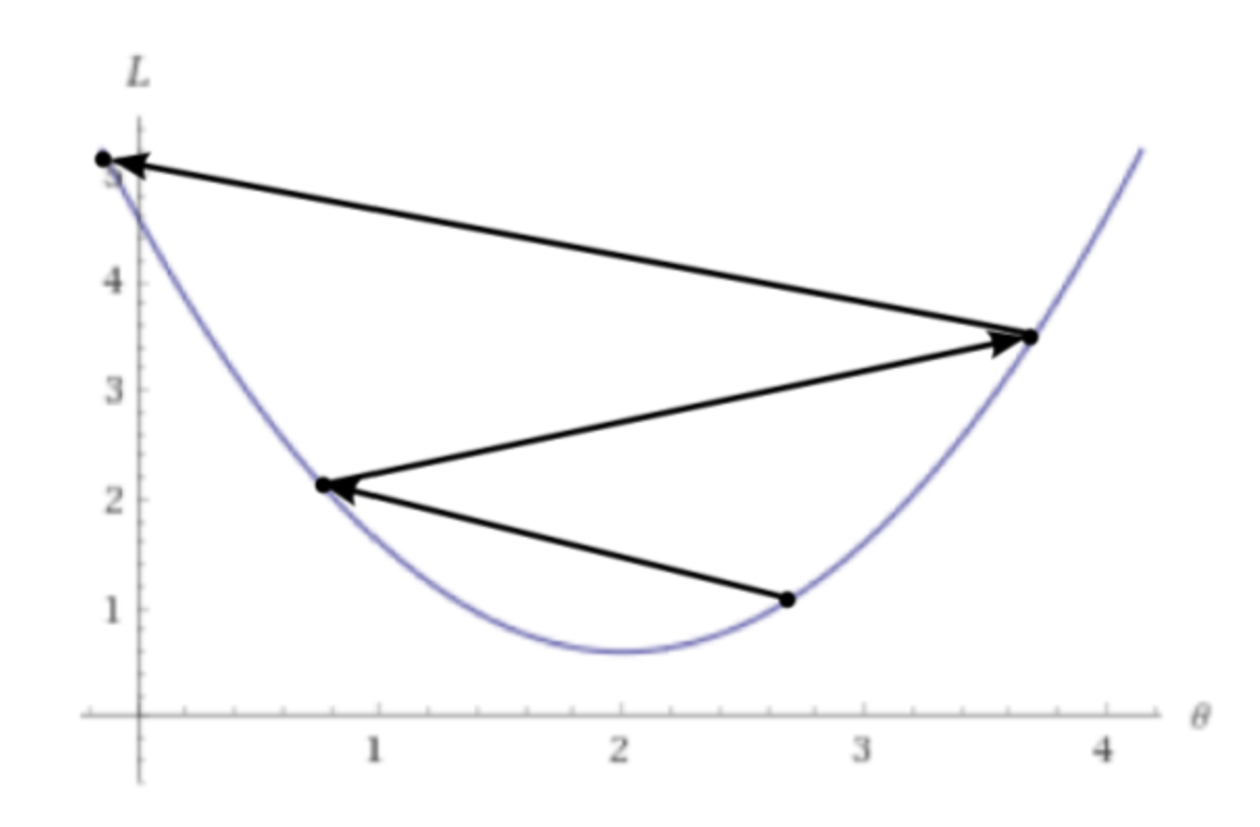
\includegraphics[width=0.8\textwidth]{Cap3/gddivergence.eps}
	\caption{ Illustration Gradient Descent divergence for a one variable optimization.
		\cite{tgilharco}.
	}
	\label{fig:gddivergence}
\end{figure}

In practice, learning works well even when some of these requirements are not met. In the context of Deep Learning, it is difficult to analyze if a function is convex because it depends on thousands or millions of parameters. Furthermore, there are activation functions themselves that are not differentiable in the whole interval it acts. Finally, the learning rate that the theorem guarantee convergence is too small. Therefore, it is common to search for a learning rate that converges faster. 

Adaptive learning rate is another technique used for make convergence faster.


\begin{gdconv}
	Suppose the function $f : \mathbb{R}^{n} \rightarrow \mathbb{R}$ is convex and differentiable, and that its gradient is Lipschitz continuous with constant $L > 0$, i.e, we have that $\lVert \nabla f(x) - \nabla f(y) \rVert_{2} \leq L\lVert x - y \rVert_{2}$, for any x, y. Then if we run gradient descent for k iterations with a adaptive step $t_{i}$, chosen using backtracking line search on each iteration $i$, it will yield a solution $f^{(k)}$ which satisfies
	
	\begin{equation}
	f(x^{(k)}) - f(x^{(*)}) \leq \frac{\lVert x^{(0)} - x^{*} \rVert^{2}_{2}}{2t_{min}k} 
	\end{equation}
	
	where $t_{min} = \min({1, \beta / L})$.
\end{gdconv}


Intuitively, using an adaptive learning rate, we can use larger initial values and then speedup learning. The most common method is learning rate decay, which could be linear, exponential.

In this work, we will use linear learning rate decay.